\documentclass[a4paper,12pt]{article}
\usepackage[utf8]{inputenc}
\usepackage[cm,empty]{fullpage}
\usepackage[T2A]{fontenc}
\usepackage[english, russian]{babel}
\usepackage{amssymb,amsmath,amsxtra,amsthm}
\usepackage{proof}
\usepackage[pdftex]{graphicx}
\usepackage{wrapfig}
\usepackage{braket}
\usepackage{xcolor}
\usepackage{enumitem}

\usepackage[left=2cm,right=2cm,
    top=1cm,bottom=1cm,bindingoffset=0cm]{geometry}

\renewcommand{\leq}{\leqslant}
\renewcommand{\geq}{\geqslant}


\newcommand{\iiff}{\Longleftrightarrow}
\renewcommand{\iff}{\Leftrightarrow}
\newcommand{\nothing}{\varnothing}

\newtheorem*{rem}{Замечание}

\newcommand{\NN}{\mathbb{N}}
\newcommand{\ZZ}{\mathbb{Z}}
\newcommand{\Q}{\mathbb{Q}}
\newcommand{\A}{\mathbb{A}}
\newcommand{\R}{\mathbb{R}}
\renewcommand{\C}{\mathbb{C}}

\renewcommand{\phi}{\varphi}
\newcommand{\eps}{\varepsilon}

\makeatletter
\newcommand*{\rom}[1]{\expandafter\@slowromancap\romannumeral #1@}
\makeatother

\newcounter{z}


\newcommand{\zs}{\refstepcounter{z}\vskip 10pt\par\noindent
\fbox{\textbf{12.\arabic{z}}} }

\newcommand{\z}{\refstepcounter{z}\vskip 20pt\noindent
\fbox{\textbf{\arabic{z}}} }

\renewcommand{\date}{{\bf 7 мая 2021}} 

\newcommand{\dif}
{
------------------------------------------------------------------------------------------------------------------------------------------------------
}

\newcommand{\HSEhat}{
\vspace*{-0pt}
\noindent
\setcounter{z}{0}


{\bf \phantom{\date}  \large \hfill Теория вероятностей: \hfill \normalsize \date}

\vspace{5 pt}
{\bf \large \hfill  лекция 2\hfill }

\vspace{15 pt}
\centerline{ \large  Домашнее задание.}
\centerline{ \large  Кирилл Сетдеков}



\vspace*{10pt}
\setcounter{z}{0}

}

\begin{document}
\HSEhat


\begin{enumerate}

\subsection*{Задачи:}



\item Докажите первые три свойства математического ожидания (МО от константы, МО от случайной величины умноженной на константу и МО суммы двух случайных величин)\\
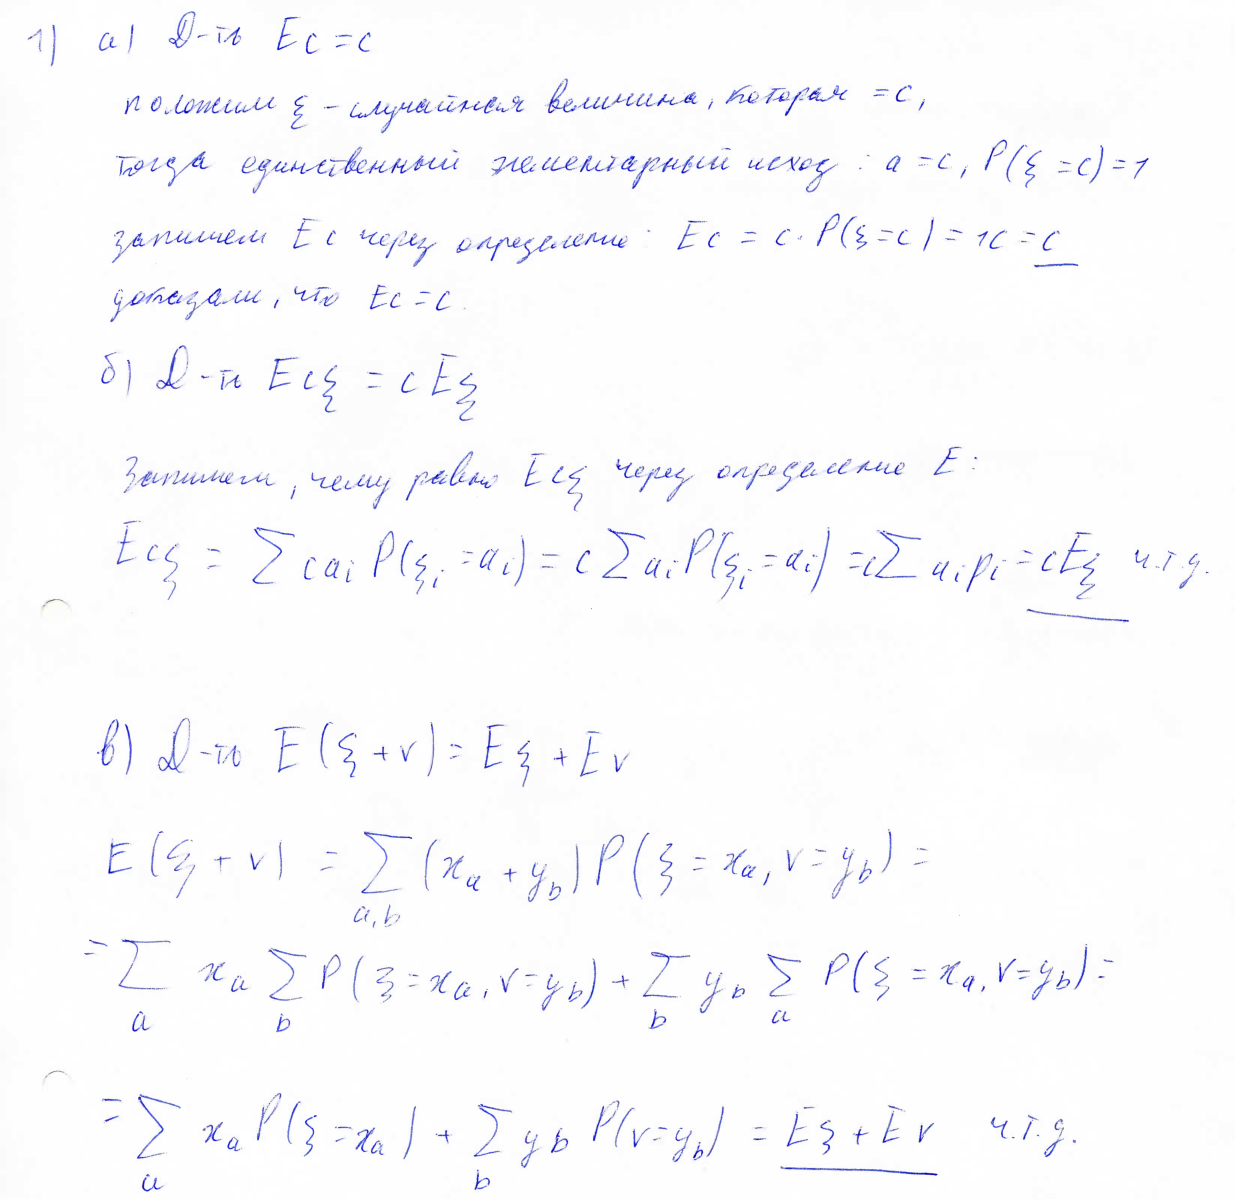
\includegraphics[width=\textwidth]{img/img207.pdf}

\item Докажите следующие свойства дисперсии: Дисперсия константы, дисперсия от случайной величин, умноженной на константу и Дисперсия случайной величины к которой добавили константу\\
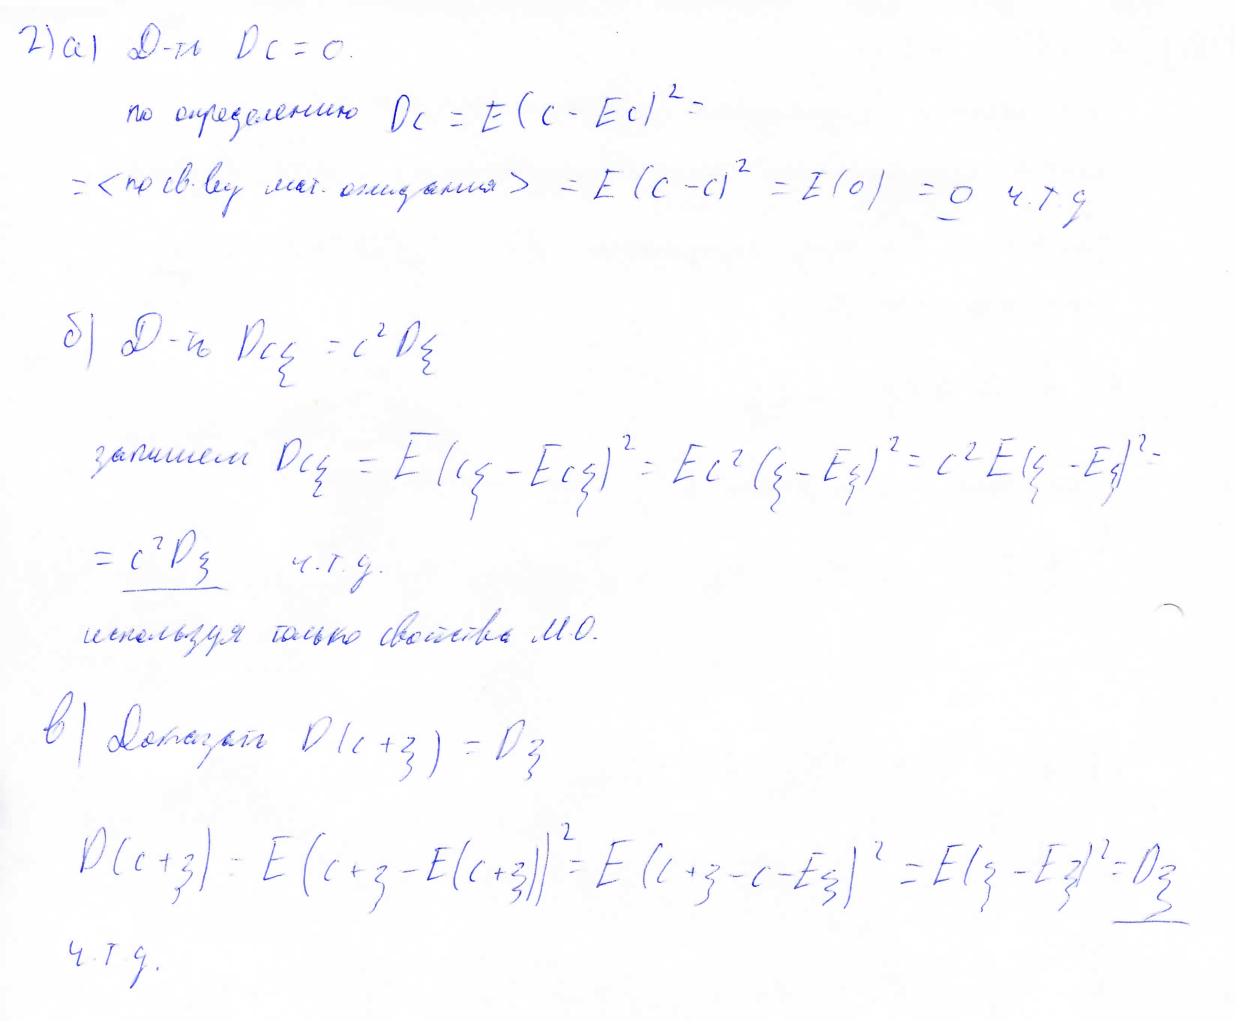
\includegraphics[width=\textwidth]{img/img208.pdf}
\item Распределение случайной величины задано таблицей


\begin{center}
 \begin{tabular}{|c| c| c| c|c|} 
 \hline
 $\xi$ & -1 & 0 & 4 & 15 \\ 
  \hline
 $\xi^2$ & 1 & 0 & 16 & 225 \\ 
 \hline
 P & 1/10 & 1/3 & 1/2 & 1/15 \\ 
 \hline
\end{tabular}
\end{center}
Найдите МО и дисперсию

\textbf{Решение:}\\
Допишем в таблице выше значения $\xi^2$

$$E(\xi)=\sum_i^{4} {\xi_i P_i} = -\frac{1}{10}+0+2+1=2.9$$
$$D(\xi)=E(\xi^2) - (E(\xi))^2=\sum_i^{4} {\xi^2_i P_i}-2.9^2 = 0.1+0+8+15-8.41=14.69$$
\textbf{Ответ: МО: $2.9$, дисперсия: $14.69$}


\item У человека в кармане 6 похожих друг на друга ключей. Только один открывает дверь. Человек последовательно достает ключ и пробует открыть дверь, если не получается, то убирает ключ в другой карман. Сколько в среднем придется попробовать ключей, прежде чем получится открыть дверь\\
\textbf{Решение:}\\

Только один ключ из 6 открывает дверь. Построим случайную величину $k=$ число взятых ключей, которое мы взяли чтобы открыть дверь.
Представим, что мы открыли дверь первым ключём, вероятность этого:
$$P(k=1) = \frac{1}{6}$$
Для следующих ключей, вероятность равна произведению вероятности не открыть меньшим числом ключей на вероятность открыть последним ключём
$$P(k=2) = (1-\frac{1}{6})\frac{1}{5}=\frac{5}{6}\frac{1}{5}=\frac{1}{6}$$
$$P(k=3) = \frac{5}{6}(1-\frac{1}{5})\frac{1}{4}=\frac{5}{6}\frac{4}{5}\frac{1}{4}=\frac{1}{6}$$
$$P(k=4) = \frac{5}{6}\frac{4}{5}(1-\frac{1}{4})\frac{1}{3}=\frac{5}{6}\frac{4}{5}\frac{3}{4}\frac{1}{3}=\frac{1}{6}$$
$$P(k=5) = \frac{5}{6}\frac{4}{5}\frac{3}{4}(1-\frac{1}{3})\frac{1}{3}=\frac{5}{6}\frac{4}{5}\frac{3}{4}\frac{2}{3}\frac{1}{2}=\frac{1}{6}$$
$$P(k=6) = \frac{5}{6}\frac{4}{5}\frac{3}{4}\frac{2}{3}(1-\frac{1}{2})1=\frac{5}{6}\frac{4}{5}\frac{3}{4}\frac{2}{3}\frac{1}{2}1=\frac{1}{6}$$

Запишем ее значения и вероятности этих исходов:
\begin{center}
 \begin{tabular}{|c| c| c| c|c|c|c|} 
 \hline
 $k$ & 1 & 2 & 3 & 4 & 5& 6\\ 

 \hline
$P$ & 1/6 & 1/6 & 1/6 & 1/6 & 1/6& 1/6\\ 
\hline
\end{tabular}
\end{center}

Из расчета, приведенного в задании 8, мы уже нашли значение м.о.:
$Ek=3.5$

\textbf{Ответ: в среднем придется попробовать $3.5$ ключа}


\item Автоматический механизм производит дефектную деталь с вероятностью p. Когда это происходит, выполняется регулировка механизма. Найдите среднее число качественных деталей, производимых между регулировками.\\

\textbf{Решение:}\\
Если вероятность дефекта $p$, то вероятность, что деталь не дефектная $1-p$. Вероятность того, что деталь 2 будет не дефектная будет $p(1-p)$, так как мы хотим чтобы одновременно первая деталь была не дефектная а вторая - дефектная. Все детали независимо друг от друга могут быть дефектными. На основе этого запишем в таблицу значение дискретной с.в. $k$ , которая показывает число деталей до ремонта и вероятность этого события:
\begin{center}
 \begin{tabular}{|c| c| c| c|c|} 
 \hline
 $k$ & 1 & 2 & 3 & k\\ 

 \hline
$P$ & $p$ & $p(1-p)$ & $p(1-p)^2$ & $p(1-p)^{k-1}$\\ 
\hline
\end{tabular}
\end{center}

Запишем м.о. как бесконечную последовательность:
$$Ek = 1p+2p(1-p)+3p(1-p)^2+...+kp(1-p)^{k-1}$$
Известно, что эта последовательность сходится к $\frac{1}{p}$, следовательно
$$Ek=\frac{1}{p}$$

\textbf{Ответ: среднее число качественных деталей, производимых между регулировками $\frac{1}{p}$}


\item Из ста карточек с числами 00, 01, 02…99 наудачу вынимается одна. Пусть случайная величина $\xi$ – сумма цифр на карточке, а $v$ – произведение цифр на карточке. Найдите МО и дисперсию каждой случайной величины

\textbf{Решение:}\\

Введем еще одну случайную величину - $b$, которая принимает значения от 0 до 9 с вероятностью 1/10. Мы можем свести решение исходной задачи к нахождению $Eb$, $Db$ и из них найти МО и дисперсию для $\xi$ и $v$.

Запишем значения и вероятности для случайной величины $b$:
\begin{center}
 \begin{tabular}{|c| c| c| c|c|c|c|c|c|c|c|} 
 \hline
 $b$ & 0&1 & 2 & 3 & 4&5&6&7&8&9\\ 
  \hline

 $b^2$ & 0&1 & 4 & 9 & 16&25&36&49&64&81\\ 

 \hline
$P$ & $1/10$ & $1/10$& $1/10$& $1/10$& $1/10$& $1/10$& $1/10$& $1/10$& $1/10$& $1/10$\\ 
\hline
\end{tabular}
\end{center}

$$E(b)=\sum_i^{10} {a_i P_i} = 4.5$$
$$D(b)=E(b^2) - (E(b))^2=\sum_i^{10} {b^2_i P_i}-4.5^2 = 8.25$$

По свойствам МО и дисперсии, так как первая и 2 цифра - независимые случайные величины на этих карточках:
$$E(\xi) =2E(b)= 9$$
$$D(\xi) =2D(b)= 16.5$$
$$E(v) =E(b) E(b)= 4.5^2=20.25$$
$$D(v)=E(b^2) E(b^2) - E(b))^2 E(b))^2= [E(b^2)]^2-E(b))^4 = 28.5^2-4.5^4=402.1875$$


\textbf{Ответ: для суммы: $E(\xi) = 9$, $D(\xi) = 16.5$; для произведения: $E(v) =20.25$, $D(v)=402.1875$ }


\item Аудитор обнаруживает финансовые нарушения у проверяемой фирмы с вероятностью 0,85. Найти вероятность того, что среди 8 фирм будет выявлено строго больше 6 нарушителей 

\textbf{Решение:}\\
Случайная величина $n$, которая равна выявленному числу фирм имеет биномиальное распределение с параметром $p=0.85$.

Нас интересует событие $A: n>6$\\
Оно эквивалентно объединению событий $n=7$ и $n=8$.\\
Найдем вероятность:
$$P(n=7)+P(n=8)=C^7_8p^7q+p^8=8 \cdot 0.85^7 \cdot 0.15 +0.85^8\approx0.6572$$
\textbf{Ответ: искомая вероятность: $\approx0.6572$}


\item Найти дисперсию и МО суммы очков, выпавших на n игральных костях\\
\textbf{Решение:}\\
Пусть $a$ - случайная величина, которая задает значение, которое выдает 1 кубик. Запишем ее значения, вероятности и $a^2$, чтобы посчитать $E(a); D(a)$
\begin{center}
 \begin{tabular}{|c| c| c| c|c|c|c|} 
 \hline
 $a$ & 1 & 2 & 3 & 4 & 5& 6\\ 
 \hline
  $a^2$ & 1 & 4 & 9 & 16 & 25& 36\\ 
 \hline
$P$ & 1/6 & 1/6 & 1/6 & 1/6 & 1/6& 1/6\\ 
\hline
\end{tabular}
\end{center}
$$E(a)=\sum_i^{6} {a_i P_i} = \frac{28}{6}=\frac{7}{2}=3.5$$
$$D(a)=E(a^2) - (E(a))^2=\sum_i^{6} {a^2_i P_i}-\frac{7^2}{2^2} = \frac{91}{6}-\frac{49}{4}=\frac{35}{12}=2\frac{11}{12}$$

По свойству МО: $E(n a) = nE(a) = \frac{7}{2}n$\\
По свойству дисперсии, учитывая, что результаты кубиков независимы:\\ $D(\sum^n a) = n D(a) = 2\frac{11}{12}n$\\
\textbf{Ответ: Дисперсия: $2\frac{11}{12}n$, МО: $3\frac{1}{2}n$}


\end{enumerate}
\end{document}